\documentclass[12pt, a4paper]{article}

\usepackage[utf8]{inputenc}
\usepackage[greek, english]{babel}
\usepackage{alphabeta}
\usepackage{libertine}
\usepackage{graphicx}
\usepackage{biblatex}[sorting=nty] % sort alphabetically
\usepackage[table]{xcolor}
\usepackage{lipsum}
\usepackage{hyperref}

\graphicspath{ {./resources/} }
\addbibresource{refs.bib}

\def\code#1{\texttt{#1}}

\title{\Huge Content-based vs Collaborative Recommendation Systems: A Brief Comparison }

\author{\LARGE Tsirmpas Dimitris\\Athens University of Economics and Business\\Department of Informatics}

\begin{document}

\pagenumbering{gobble}
\maketitle

\begin{center}
    
\includegraphics[width=1\textwidth]{aueb_logo.jpg}
    
    \LARGE Professor: Sarantopoulos Panagiotis
    
    \large Athens University of Economics and Business
    
    \large Department of Business Administration
    
    \large Greece
    \newpage
    
\end{center}

\pagenumbering{arabic}

\begin{abstract}
    Recommendation systems have become omnipresent in our everyday lives and necessary for most corporations. However, different kinds of recommendation systems exist offering unique advantages, challenges and limitations. In this short report, we describe and compare two of the most popular such systems; Content-based and Collaborative filtering, as well as their shared weaknesses. Understanding the characteristics of the respective systems helps managers make informed decisions for their specific business requirements.
\end{abstract}


\section{Introduction}
Recommendation systems have become almost a necessity in the modern era of e-commerce. These systems, used from movies \cite{movie1}, to music \cite{music1, music2}, news \cite{news1}, tangible commercial products \cite{commerce1, commerce2}, to even scientific articles \cite{scientific1}, have proven extremely sought after in today's era of digitization, information and big data. Besides practical and monetary benefits, they also represent a constantly evolving area for the application of new statistical and machine-learning models, attracting the attention of much of the scientific community.

Traditionally, two of the most successful recommendation systems were \textbf{Content-based} (CB) and \textbf{Collaborative} filtering (CF). They both attempt to find new items to recommend to a user based on information on the items themselves and the user's recorded purchase (when applied to e-commerce) history. Where they differ, is the kind of information used, where CB systems look into the previously purchased items and CF into the users who have purchased similar items. While these systems were traditionally implemented using standard statistical procedures, the advent of neural networks has greatly impacted the capabilities, implementation and use of these systems. 

In this short report we will compare the two types, outlining advantages, disadvantages and similarities. This report does not require any technical depth on the part of the reader, since we intend this to be a short primer for managers and consultants on recommendation systems.


\section{Common challenges}

Most recommendation systems face a number of generic challenges which are caused by the nature of the common problem they seek to solve. Some of the most important ones include:

\begin{itemize}
    \item \textbf{The cold start problem}. Since recommendation systems are based on utilizing information about the user and the items he interacts with, when information about either the user, or the items themselves, or both, are unavailable (new or inactive users, new or unpopular products), the system struggles to make any recommendation \cite{cold-start}.

    \item \textbf{Data sparsity}. A generalization of the cold start problem, where our system is unable to find patterns because of insufficient data, or because of the presence of too many user/item attributes (called \textit{"the curse of dimensionality"} in formal statistic and machine learning circles). In the second case, as we consider more and more features to attach to our users and items, the amount of data we need to back our system increases exponentially. This can be seen in Figure \ref{fig:cod}.

    \item \textbf{Originality}. Recommendation systems have a tendency to prioritize "safe", popular and highly rated items over items which the user might have not thought of themselves. This inhibits our systems learning patterns from our users and limits their potential. Some authors \cite{survey2} stress the difference between simply "novel" recommendations, and truly surprising ones.

    \item \textbf{Shilling attacks}. Since recommendation systems are mostly used for monetary benefit, there is a strong incentive for bad actors to attempt to influence them into promoting or hiding particular items.

    \item \textbf{Privacy}. Obtaining detailed information about the user is essential for any recommendation system. However, different legal frameworks restrict the amount of such information that can be obtained.

    \item \textbf{Scalability}. Any algorithm with a linear ($O(N)$) or higher complexity will struggle to perform at all in large datasets. Complexity here means that as the size of a problem increases, the time or resources needed to solve it also increases in a direct and consistent manner. In datasets using potentially tens of millions of users or products, algorithms that don't account for those data sizes, will not be usable.

\end{itemize}

\begin{figure}
    \centering
    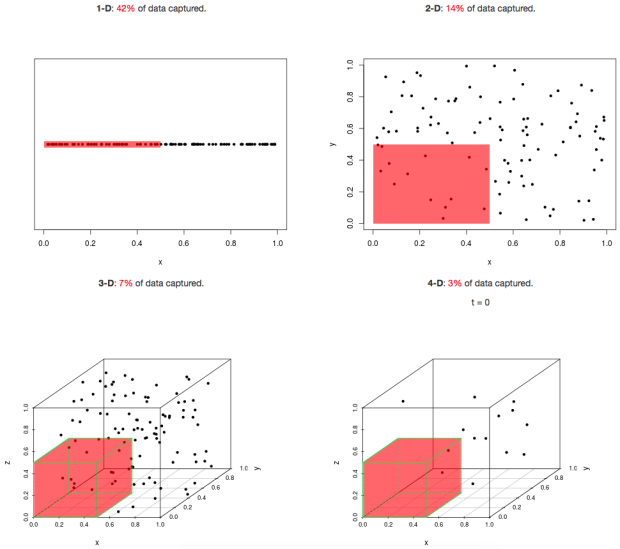
\includegraphics[width=8cm]{resources/COD.png}
    \caption{A visualization of a dataset suffering from the curse of dimensionality. Note how the more dimensions we view our data, the less data there are to observe. Image credits: (\href{https://eranraviv.com/curse-of-dimensionality/}{Eran Raviv}).}
    \label{fig:cod}
\end{figure}


\section{Content-based Filtering}

Content-based filtering is a prominent technique employed in information retrieval and recommendation systems to personalize content recommendations for users. It relies on the inherent characteristics and properties of the items themselves, such as textual features or metadata, to establish similarity measures between items. By analyzing the content of items that a user has already interacted with, content-based filtering algorithms identify other items with comparable attributes to recommend. 

CB systems can be categorized in two main categories:
\begin{itemize}
    \item \textbf{Memory-Based} systems, which query an extensive dataset (usually in a database), and attempt to find patterns by utilizing similarity metrics such as Pearson's coefficient or cosine similarity.

    \item \textbf{Model-based} systems, which "encode" the dataset in an ideal, internal representation which is used to make predictions by a model. The model in this case usually is a machine learning algorithm.
\end{itemize}

The main advantages of a CB system are \cite{survey1, survey2}:
\begin{itemize}
    \item Their results can be more personalized, since they are independent of other users.
    \item They are easy to interpret, making explaining the results to a user easy.
    \item They can recommend products not picked by other users (e.g brand-new or unpopular products).
\end{itemize}

The disadvantages of a CB system are \cite{survey1, survey2}:
\begin{itemize}
    \item Modelling and selecting the attributes of an item in order for the system to properly "understand" it, is difficult.
    \item The system is prone to overfitting to its own predictions, since its predictions are used to drive future ones.
    \item Verifying the performance of a CB system is difficult. Accuracy metrics exist, but only in an offline environment \cite{comparison1, comparison2}.
\end{itemize}

Additionally, \textcite{comparison2} seem to indicate that CB system tend to select different items when in small recommendation lists than CF algorithms, although their results tend to converge the bigger these lists become. Their results also show that CB algorithms tend to be more robust, as the CF algorithms tended to struggle in datasets with many items but low user collaboration. 

Furthermore we believe that the issue of feature selection and representation may be solved by modern neural network architectures, which have the ability to learn their own representations from raw data. For instance, while traditional CB models relied on "manual" representations for text, advancements in Natural Language Processing (NLP) could drastically improve the quality of the data that can be automatically extracted from product titles and descriptions.


\section{Collaborative Filtering}

This approach relies on the collective "wisdom" of a user community by analyzing their past behaviors and preferences,as opposed to the items themselves. Through the identification of similar users or items, collaborative filtering algorithms seek to generate recommendations for a target user based on the experiences and choices of other like-minded individuals. By leveraging user-item interaction data, such as ratings or purchase history, collaborative filtering algorithms establish patterns of user behavior and establish relationships between users or items. Similarly to CB systems, CF systems are divided to \textbf{memory-based} and \textbf{model-based} in an identical fashion.

The main advantages of a CF system are \cite{survey1, survey2}:
\begin{itemize}
    \item Easier implementation (especially for memory-based systems).
    \item Memory-based systems are much easier to incrementally enrich with new data.
    \item Can discover more complex patterns than CB systems, since it relies on the behavioral patterns of other humans. 
\end{itemize}

The disadvantages of a CF system are \cite{survey1, survey2}:
\begin{itemize}
    \item Especially vulnerable to the \textit{cold start problem}.
    \item The \textbf{grey sheep} problem, where some users do not fit in any of the categories discovered by our system.
    \item Due to the enormous amounts of users compared to products, CF algorithms are much less scalable.
    \item Ratings are only attributed sparsely and in a small subset of all products, leading to data sparsity issues.
\end{itemize}

\textcite{comparison1} claim that hybrid recommendation systems can alleviate most of the issues of CF systems. Hybrid systems are systems using a combination of CB and CF algorithms (although other recommendation systems can be mixed as well), either by using both of their recommendations for predictions, using one's recommendations to train the other or by combining their inputs. Additionally, they have become an intense field of study for the application of neural networks \cite{nn1}, leveraging the expressive power of neural network architectures, allowing them to combine knowledge of traditionally CB and CF exclusive information.


\section{Conclusions}

Recommendation systems play a vital role in various domains, and understanding the different types of systems is crucial. Content-based filtering focuses on the attributes of items and recommends similar items based on user preferences, while collaborative filtering relies on user behavior to find like-minded individuals and generate recommendations. Both approaches have shared weaknesses, such as the cold start problem, data sparsity, and scalability issues. There is no ideal system, nor is either of the two systems more effective than the other, meaning that the prospective manager must thus make an informed decision, based on the nature of their business and data. 

\printbibliography

\end{document}
